%Preámbulo:  
\documentclass{aa} %O cualquier otra clase.
\usepackage[center]{caption}
\usepackage{hyperref}
\hypersetup{
    colorlinks=true,
    linkcolor=blue,
    filecolor=magenta,      
    urlcolor=cyan,
    pdftitle={Overleaf Example},
    pdfpagemode=FullScreen,
    }
\title{Estudio espectroscópico de una estrella problema}
\subtitle{Determinación del tipo espectral, radio y distancia}
\author{Luis Lucas García}
\institute{Universidad de Alicante}
\date{\today}
\abstract{El objetivo de esta práctica es la obtención de características de tres estrellas a partir de su información espectroscópica. Para ello vamos a utilizar la suite de StarLink, más específicamente el programa DIPSO. Obtendremos para las dos estrellas problemas su tipo espectral, su radio y su distancia con sus respectivos errores. También vamos a obtener otra información como la luminosidad.}
\keywords{Técnicas: espectroscopía - Estrellas: variables: generales}
\bibpunct{(}{)}{;}{a}{}{,}
\begin{document}
\maketitle
\tableofcontents

\section{Introducción}

\subsection{Motivación y objetivos}

La espectrometría es una técnica altamente potente capaz de permitirnos obtener parámetros estelares de diversos objetos gracias a la medida de la cantidad de luz que nos llega de ellos. Esta determinación es de suma utilidad para probar nuestros modelos estelares, así como para conocer el Universo que nos rodea.

El objetivo de esta práctica es la determinación de los parámetros de tres estrellas problema a través del análisis de sus espectros. A lo largo de la práctica obtendremos el radio, la luminosidad, la temperatura efectiva, etc. de estas estrellas.

\subsection{Fundamento teórico}

La espectrometría es la medida de la cantidad de fotones que observamos de un objeto. Midiendo esta cantidad así como sus longitudes de onda podemos hacer varios cálculos de las propiedades del objeto observado. Quizás la más útil sea la clasificación espectral de la estrella, que es como aparece en la siguiente tabla: \cite{handbook}

\begin{center}
\begin{tabular}{ccccc}
\hline \hline
Tipo esp. & $M_V$ & $(B-V)_0$ & $T_{eff} (K)$ & $L (L_{\odot})$ \\ \hline
O5 - 7 & $-5.5$ & $-0.32$ & $38000$ & $4.2 \times 10^5$ \\
B0 & $-4.0$ & $-0.30$ & $30000$ & $5.2 \times 10^4$ \\
A0 & $+0.6$ & $0.00$ & $10800$ & $54$ \\
F0 & $+2.7$ & $+0.31$ & $7240$ & $6.5$ \\
G0 & $+4.4$ & $+0.58$ & $6000$ & $1.5$ \\
K0 & $+5.9$ & $+0.81$ & $5250$ & $0.42$ \\
M0 & $+8.8$ & $+1.40$ & $3850$ & $7.7 \times 10^{-2}$ \\ \hline \hline
\end{tabular}
\captionof{table}{Propiedades promedio de estrellas en secuencia principal en función de su clasificación espectral.}
\label{table:spectral}
\end{center}

Una vez conocido el tipo espectral de nuestra estrella necesitamos ecuaciones que nos permitan calcular las propiedades de nuestras estrellas.

Así pues, consultando los apuntes \cite{apuntes} de clase de astrofísica podemos determinar, por ejemplo, el enrojecimiento:

\begin{equation}
E(B - V) = (B - V) - (B - V)_0
\label{eq:reddening}
\end{equation}

Pero, con el programa lo que podemos medir son los flujos $f_B$ y $f_V$, que son las magnitudes aparentes. Si queremos la diferencia de las magnitudes absolutas tenemos que aplicar la siguiente ecuación:

\begin{equation}
(B-V) = -2.5 \, log \left( \frac{f_B}{f_V} \right) + 0.61
\end{equation}

Y con el enrojecimiento podemos determinar otras magnitudes de utilidad como la extinción o la magnitud corregida.

\begin{equation}
A_V = 3.1 E(B - V)
\end{equation}

\begin{equation}
V_0 = V - A_V
\end{equation}

Con lo que podemos determinar la distancia a la estrella considerada en parsecs (pc):

\begin{equation}
(V_0 - M_V) = 5 log \, d - 5
\end{equation}

Donde el término de la izquierda se conoce como el módulo de distancia.

También podemos determinar propiedades en magnitudes solares gracias a la siguiente ecuación:

\begin{equation}
\frac{R}{R_{\odot}} = \left( \frac{T_e^{\odot}}{T_e} \right)^2 \left( \frac{L}{L_{\odot}} \right)^{\frac{1}{2}}
\label{eq:apuntes}
\end{equation}

Sabemos que el Sol es una estrella de tipo G2V \cite{encyclopedia} por lo que podemos tomarle una temperatura efectiva de 5777K.

Nuestro objetivo será la obtención de los espectros, el tipo espectral, radio, luminosidad, etc. de las dos estrellas problemas. También intentaremos identificarlas con algunas estrellas de su mismo tipo espectral con características conocidas.

\section{Desarrollo experimental}

Vamos a trabajar con la suite de StarLink, más específicamente con el programa de DIPSO. Este programa nos permitirá realizar el análisis de los espectros de las estrellas problema.

Para el estudio contamos con dos espectros sin tratar de dos estrellas problemas. Podemos normalizar estos espectros para obtener lo que se observa en la figura \ref{fig:espectroNorm}

\begin{figure}[h!]
\begin{center}
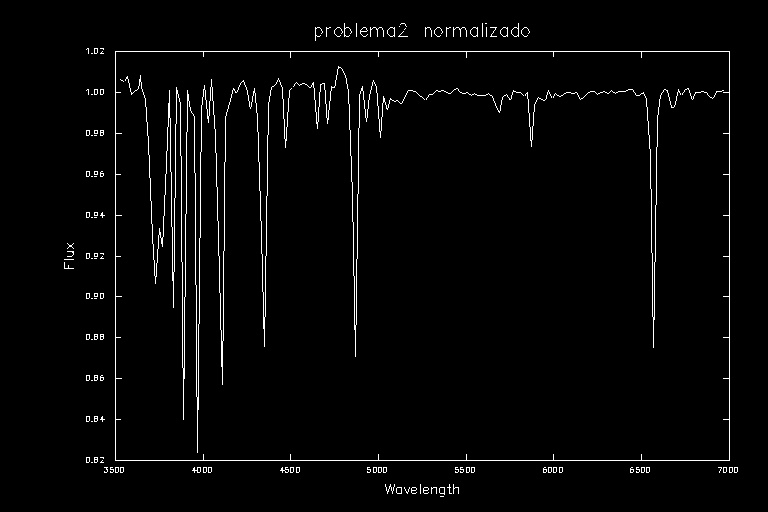
\includegraphics[scale=0.15]{Problema2 normalizado.png}
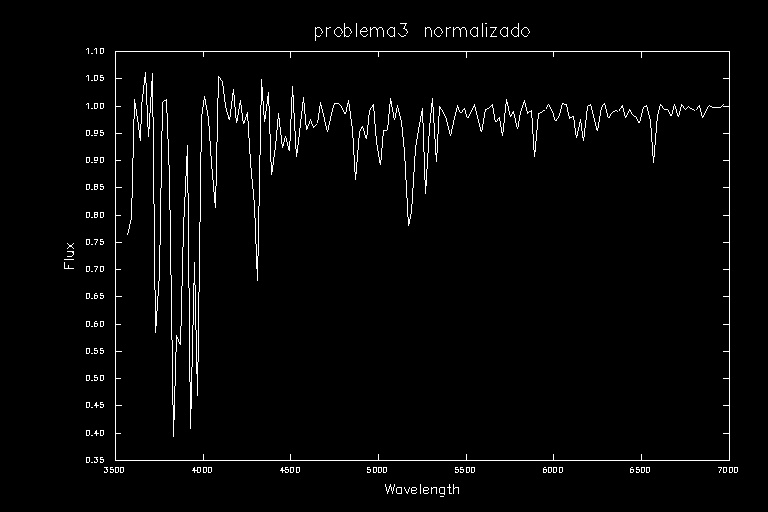
\includegraphics[scale=0.15]{Problema3 normalizado.png}
\caption{Espectros normalizados de las dos estrellas problema.}
\label{fig:espectroNorm}
\end{center}
\end{figure}

También vamos a trabajar la estrella que se nos da de ejemplo, como vemos su espectro normalizado en la figura \ref{fig:espEj}.

\begin{figure}[h!]
\begin{center}
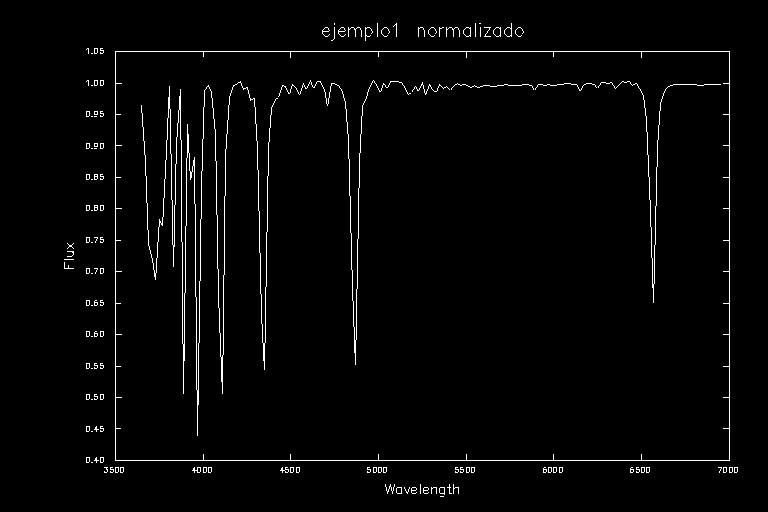
\includegraphics[scale=0.3]{1 normalizado.png}
\caption{Espectro de la estrella ejemplo 1 normalizado.}
\label{fig:espEj}
\end{center}
\end{figure}

Ya que tenemos las curvas normalizadas podemos comparar estas gráficas junto a las de una estrella genérica de cada tipo espectral y obtendremos las figuras \ref{fig:ajuste1}, \ref{fig:ajuste2} y \ref{fig:ajuste3} que son las que mejor se ajustan.

\begin{figure}[h!]
\begin{center}
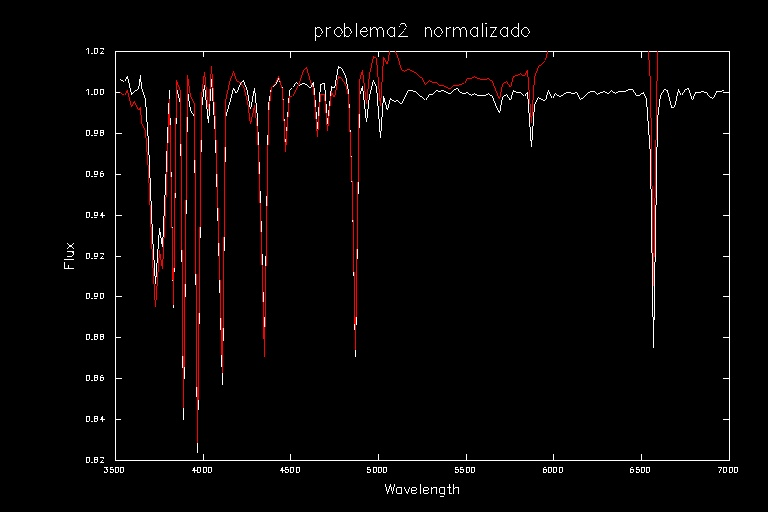
\includegraphics[scale=0.3]{2 ajustado.png}
\caption{Espectro de la estrella problema 2 comparado con el de una de tipo B0V.}
\label{fig:ajuste1}
\end{center}
\end{figure}

\begin{figure}[h!]
\begin{center}
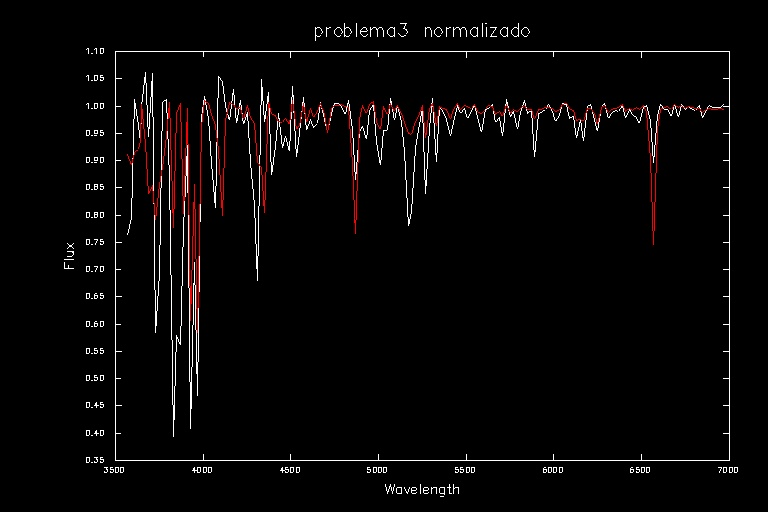
\includegraphics[scale=0.3]{3 ajustado.png}
\caption{Espectro de la estrella problema 3 comparado con el de una de tipo F0V.}
\label{fig:ajuste2}
\end{center}
\end{figure}

\begin{figure}[h!]
\begin{center}
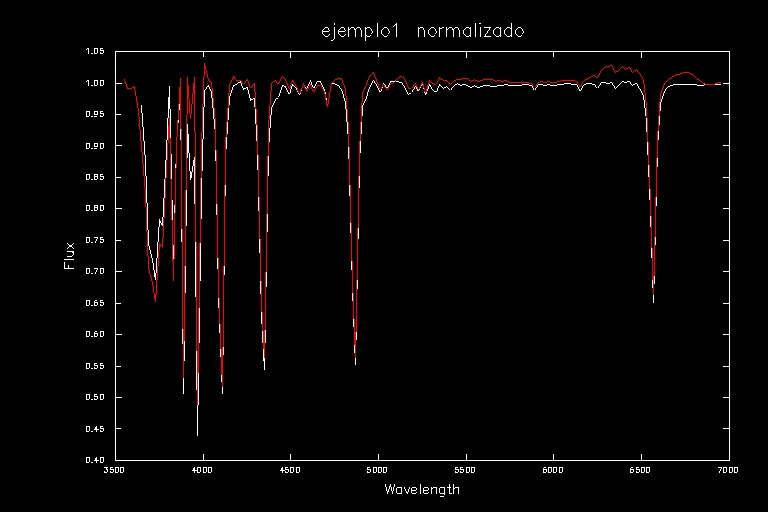
\includegraphics[scale=0.3]{1 ajustado.png}
\caption{Estrella ejemplo 1 ajustada a una estrella de tipo A0V.}
\label{fig:ajuste3}
\end{center}
\end{figure}

Luego, podemos encuadrar la estrella problema 2 con una estrella de tipo B0V mientras que la estrella problema 3 se puede relacionar con una estrella de tipo F0V y la estrella problema 1 con una de tipo A0V, lo cual nos permite conocer algunas propiedades básicas.

Lo siguiente que haremos será medir los flujos de cada estrella en los filtros B y V con su respectivo error. Suponiendo un error arbitrario en el filtro podemos obtener que para la estrella problema 2:

$$
\begin{array}{c}
f_V = (1.10000 \pm 0.00001) \times 10^{-13} \\ f_B = (7.90000 \pm 0.00001) \times 10^{-14}
\end{array}
$$

Para el caso de la estrella problema 3 tenemos que:

$$
\begin{array}{c}
f_V = (8.5600 \pm 0.0004) \times 10^{-15} \\ f_B = (3.480 \pm 0.003) \times 10^{-15}
\end{array}
$$

Y en el caso de la estrella ejemplo 1 tenemos que:

$$
\begin{array}{c}
f_V = (5.9 \pm 0.5) \times 10^{-14} \\ f_B = (5.40000 \pm 0.00004) \times 10^{-14}
\end{array}
$$

Utilizando ahora el tipo espectral de cada estrella junto con la tabla \ref{table:spectral} y la ecuación \ref{eq:reddening} podemos determinar el corrimiento al rojo de cada estrella problema y la estrella ejemplo:

$$
\begin{array}{c}
E(B - V)_2 = 1.27000 \pm 0.00001 \\ E(B-V)_3 = 1.290 \pm 0.003 \\ E(B-V)_1 = 0.73 \pm 0.09
\end{array}
$$

Podemos obtener así, haciendo uso del programa, los espectros desenrojecidos de las dos estrellas problema y el de la estrella de ejemplo.

\begin{figure}[h!]
\begin{center}
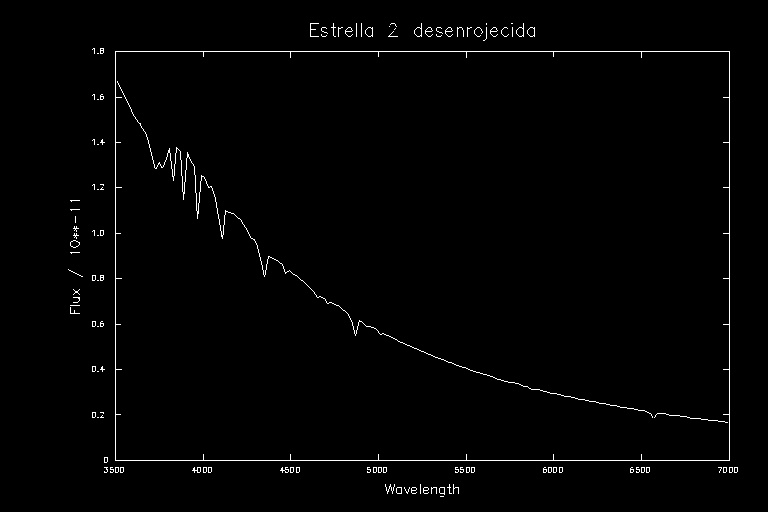
\includegraphics[scale=0.15]{2 desenrojecido.png}
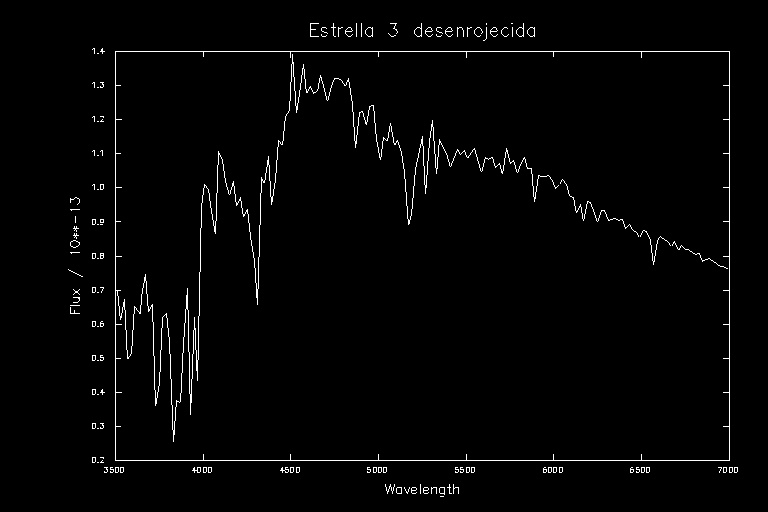
\includegraphics[scale=0.15]{3 desenrojecido.png}
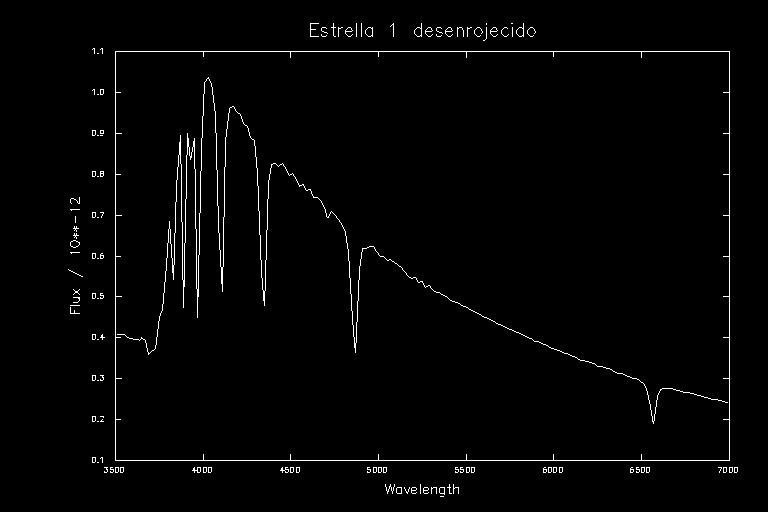
\includegraphics[scale=0.15]{1 desenrojecido.png}
\caption{Espectros desenrojecidos de las dos estrellas problema y la estrella de ejemplo.}
\label{fig:desenrojecidos}
\end{center}
\end{figure}

Podemos normalizar estos espectros y obtener una constante que no es más que $\frac{R (R_{\odot})}{d (kpc)}$, obteniendo las siguientes constantes de normalización para cada estrella.

$$
\begin{array}{ccc}
k_2 = 4.36 \, \frac{R_{\odot}}{kpc} & k_3 = 4.29 \, \frac{R_{\odot}}{kpc} & k_1 = 4.53 \, \frac{R_{\odot}}{kpc}
\end{array}
$$

\section{Análisis de resultados}

Habiendo determinado el tipo espectral de cada estrella  podemos determinar muy fácilmente algunas propiedades básicas de estas estrellas, siendo que, observamos la siguiente tabla.

\begin{center}
\begin{tabular}{ccccc}
\hline \hline
Estrella & Tipo esp. & $M_V$ & $(B-V)_0$ & $T_{eff} (K)$ \\ \hline
Ejemplo 1 & A0V & $+0.6$ & $-0.02$ & $9500$ \\
Problema 2 & B0V & $-4.0$ & $-0.30$ & $30000$ \\
Problema 3 & F0V & $+2.7$ & $+0.31$ & $7240$ \\
\hline \hline
\end{tabular}
\captionof{table}{Tabla de propiedades espectrales de las estrellas problema.}
\end{center}

Con la información espectroscópica podemos determinar la distancia a la que se encuentra cada estrella, tenemos que las distancias son:

$$
\begin{array}{cc}
d_2 = 1840.00 \pm 0.03 \, pc & d_3 = 297.0 \pm 0.4 \, pc
\end{array}
$$
$$
d_1 = 660 \pm 60 \, pc
$$

Y, usando las constantes de normalización del apartado anterior, podemos calcular los radios de estas estrellas en unidades de radios solares, siendo:

$$
\begin{array}{cc}
R_2 = 8.01000 \pm 0.00003 R_{\odot} & R_3 = 1.2800 \pm 0.0004 R_{\odot}
\end{array}
$$
$$
R_1 = 2.99 \pm 0.06 R_{\odot}
$$

Luego, usando la ecuación \ref{eq:apuntes} podemos obtener la luminosidad en unidades solares, que para las dos estrellas problemas es:

$$
\begin{array}{c}
L_2 = (4.67000 \pm 0.00001) \times 10^4 L_{\odot} \\ L_3 = 4.000 \pm 0.002 L_{\odot} \\
L_1 = 65 \pm 3 L_{\odot}
\end{array}
$$ 

Con esto hemos extraído gran parte de la información que queríamos de nuestras estrellas, lo que nos quedará ahora es ver cómo se sostienen nuestras hipótesis.

\section{Comparación de resultados}

Vamos a comenzar viendo como se comportan las hipótesis de los tipos espectrales de dichas estrellas, puesto que la luminosidad queda fuera de error vamos a comparar las luminosidades con otras clases de luminosidad dentro del mismo tipo espectral (B0 para la estrella problema 2 y F0 para la estrella problema 3. A0 para la estrella de ejemplo 1).

Los valores que se usan para cada tipo son los de la luminosidad de su estrella de referencia, es decir, por ejemplo para el tipo B0Iab consideramos la estrella $\varepsilon - Orionis$. Se pueden consultar en la bibliografía. No los cito todos porque hay bastantes referencias para las luminosidades.

\begin{figure}[h!]
\begin{center}
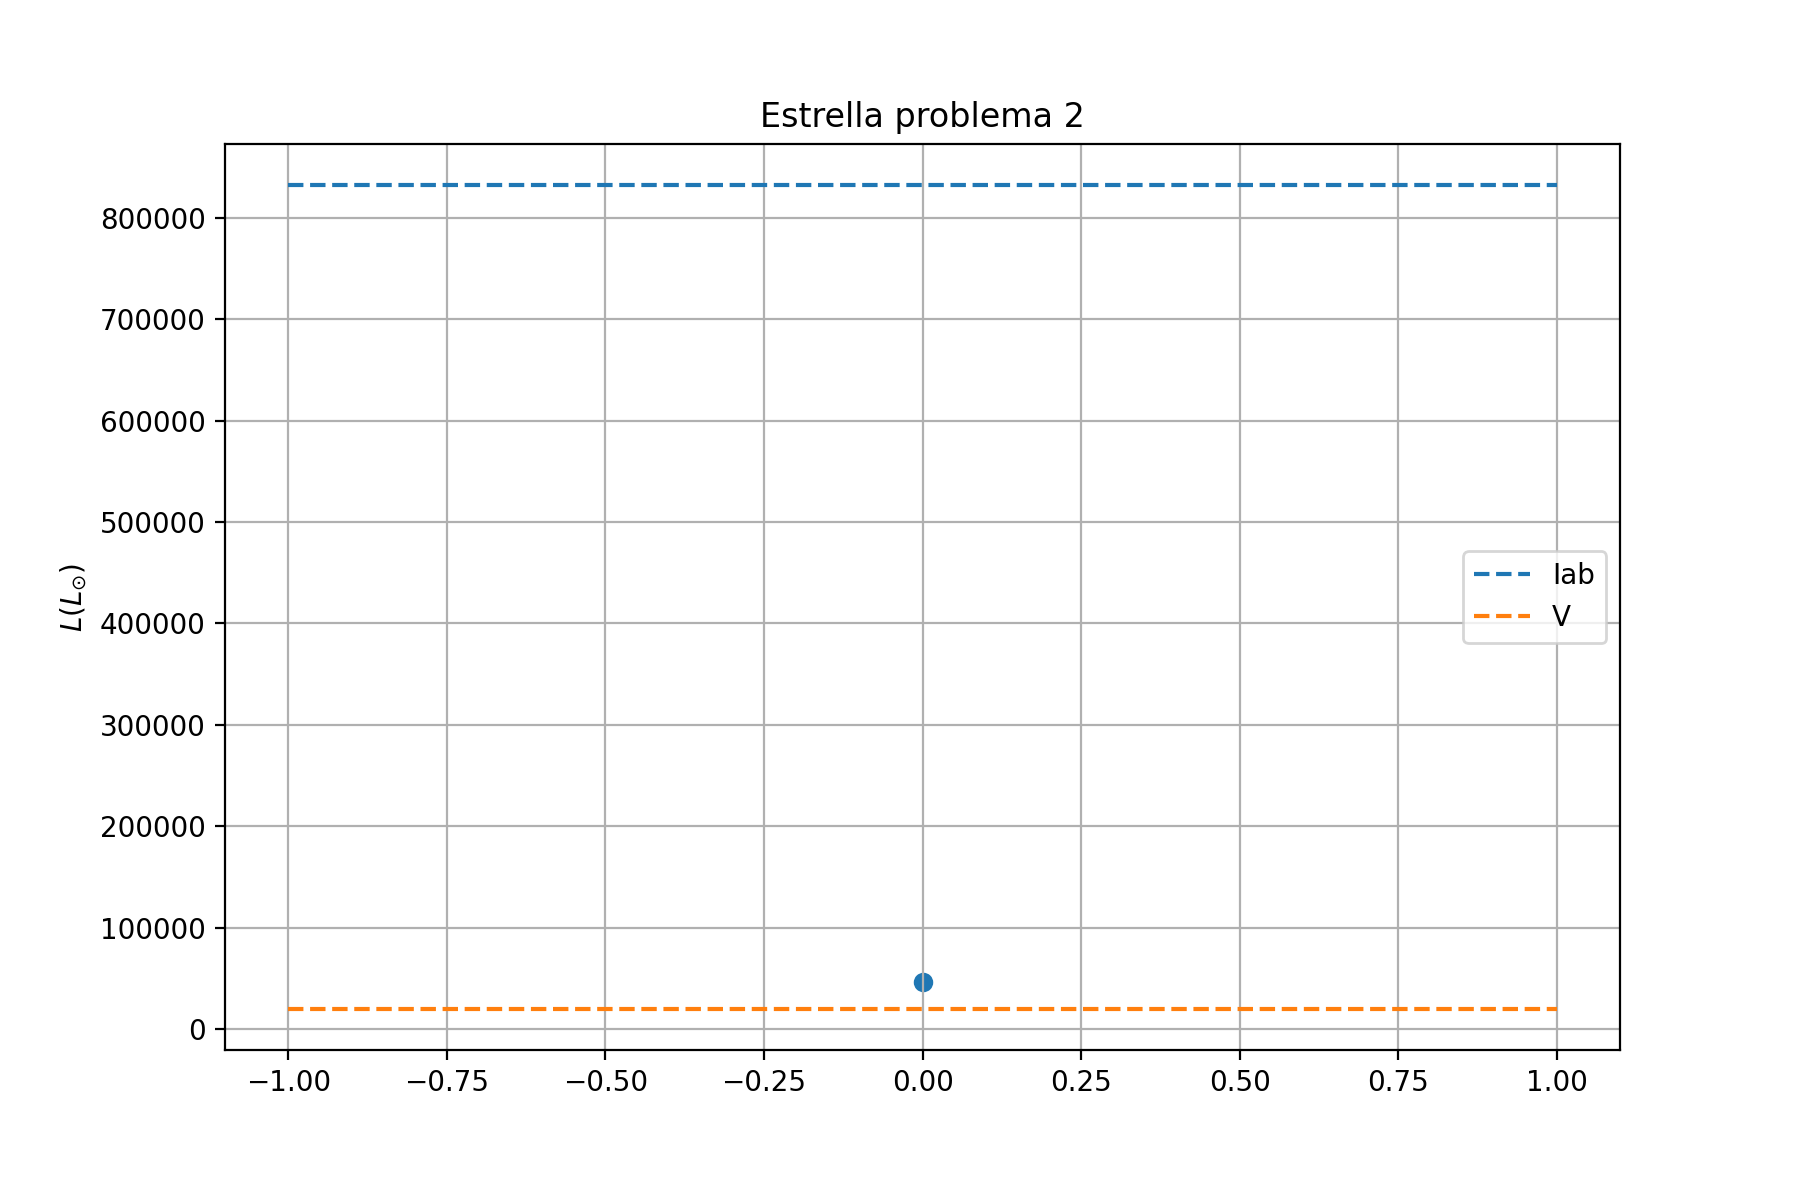
\includegraphics[scale=0.35]{TipoB.png}
\caption{Cota superior de luminosidad en el tipo B0 (\cite{Puebla_2015}) y la cota inferior (\cite{CiteDrive2022}) junto al valor de luminosidad de la estrella problema 2.}
\label{fig:tipoB}
\end{center}
\end{figure}

Como se puede observar la estrella está en el rango de luminosidades que se pueden considerar para las estrellas del tipo B0 siendo la más alta observada un orden mayor, de hecho, sería hasta correcto considerar a la estrella problema en el tipo espectral B0V.

Ya que la estrella problema 2 queda por debajo de la media de las de tipo B0V pero podemos encontrar estrellas con menos luminosidad dentro de este mismo tipo concluimos en que considerar a la estrella problema 2 de tipo B0V es correcto.

Hagamos el mismo procedimiento para la estrella problema 3, que hemos supuesto de tipo F0V, ahora, la luminosidad también está ligeramente alejada de este tipo, por lo que veamos como se comporta respecto a otras estrellas en este rango.

\begin{figure}[h!]
\begin{center}
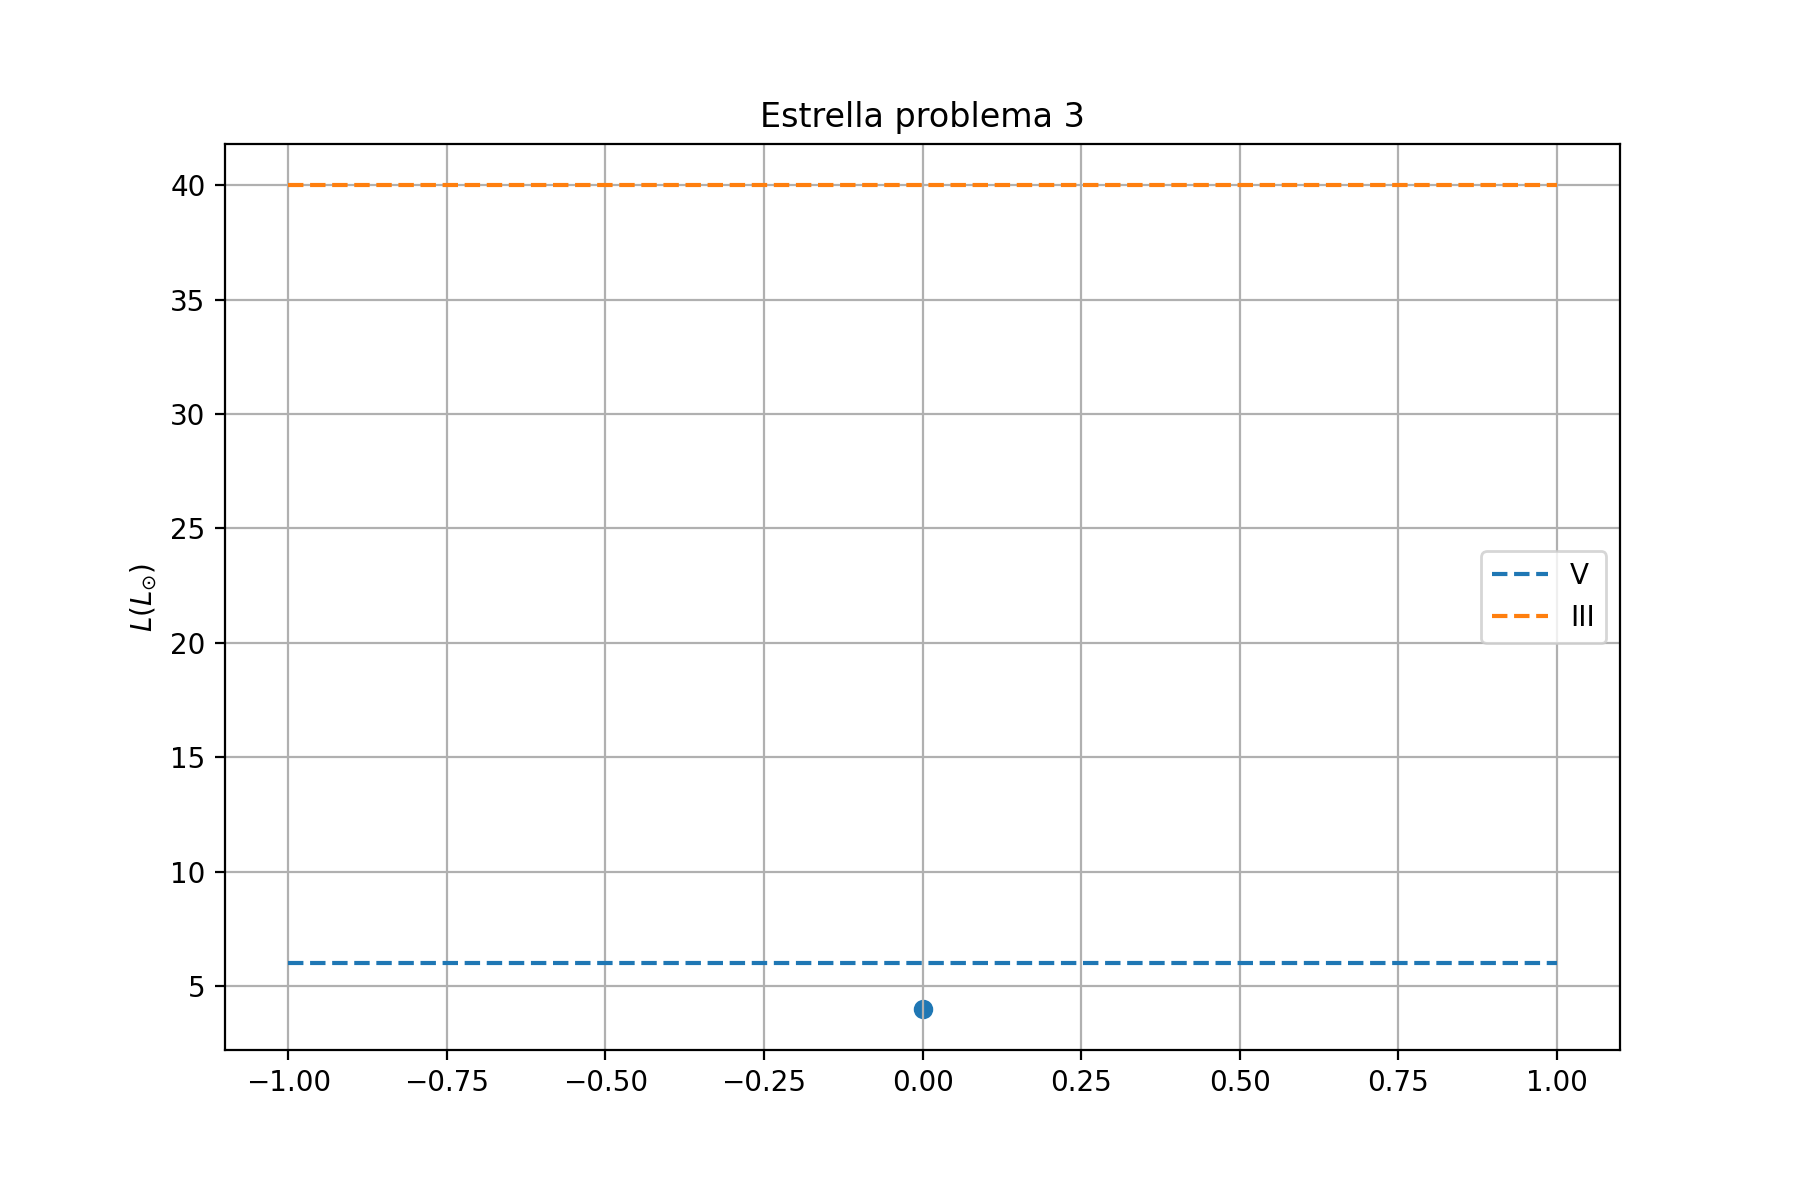
\includegraphics[scale=0.35]{TipoF.png}
\caption{Una estrella de tipo F0V y otra de tipo F0III ambas de la referencia \cite{CiteDrive2022}. También aparece marcada con un punto la estrella problema 3}
\label{fig:problema3}
\end{center}
\end{figure}

En este caso, la estrella problema 3 cae por debajo de una de tipo F0V luego quizás habría que considerar su clasificación como una estrella de tipo F0VI, una subenana, por debajo de las de la secuencia principal, aunque no mucho, aun así, la consideración en F0V no sería tampoco errónea pues no hay una distancia muy grande a la media.

La estrella de ejemplo 1 si que podemos incluirla en las de tipo A0V pues su luminosidad sí es cercana a la media de estas estrellas.

Vamos a construir ahora una tabla con la información de cada estrella, considerando también la estrella ejemplo 1. El procedimiento para esta estrella es el mismo.

\begin{center}
\begin{tabular}{cccccc}
\hline \hline
Estr. & Tipo &  $d(pc)$ & $R(R_{\odot})$ & $L(L_{\odot})$ & $T_{eff} (K)$ \\ \hline
1 & A0V & 660 & 2.99 & 65 & 9500 \\
2 & B0V & 1840 & 8.01 & $4.67 \times 10^4$ & 30000 \\
3 & F0V & 297 & 1.28 & 4 & 7200 \\ \hline \hline
\end{tabular}
\captionof{table}{Datos de las tres estrellas, la de ejemplo y las dos problemas. En la tabla \ref{tab:errores} se encuentran los valores de error para los datos que lo requieren}
\label{tab:magnitudes}
\end{center}

\begin{center}
\begin{tabular}{cccc}
\hline \hline
Estr. & $\Delta d(pc)$ & $\Delta R(R_{\odot})$ & $\Delta L(L_{\odot})$ \\ \hline
1 & 60 & 0.06 & 3 \\
2 & 0.03 & $3 \times 10^{-5}$ & 0.3 \\
3 & 0.4 & $4 \times 10^{-4}$ & $2 \times 10^{-3}$ \\
\hline \hline
\end{tabular}
\captionof{table}{Tabla con los valores del error de la tabla \ref{tab:magnitudes} que los requieran}
\label{tab:errores}
\end{center}

Podemos construir una gráfica con tres puntos para estudiar la dependencia de la luminosidad con la temperatura. En este caso esperaríamos una relación que dependa a la cuarta, siempre que mantengamos constante el radio de la estrella.

En la figura \ref{fig:TL} podemos observar como se comportan nuestras tres estrellas, así como la curva temperatura - luminosidad para distintos valores de la relación $\frac{R}{R_{\odot}}$.

\begin{figure}[h!]
\begin{center}
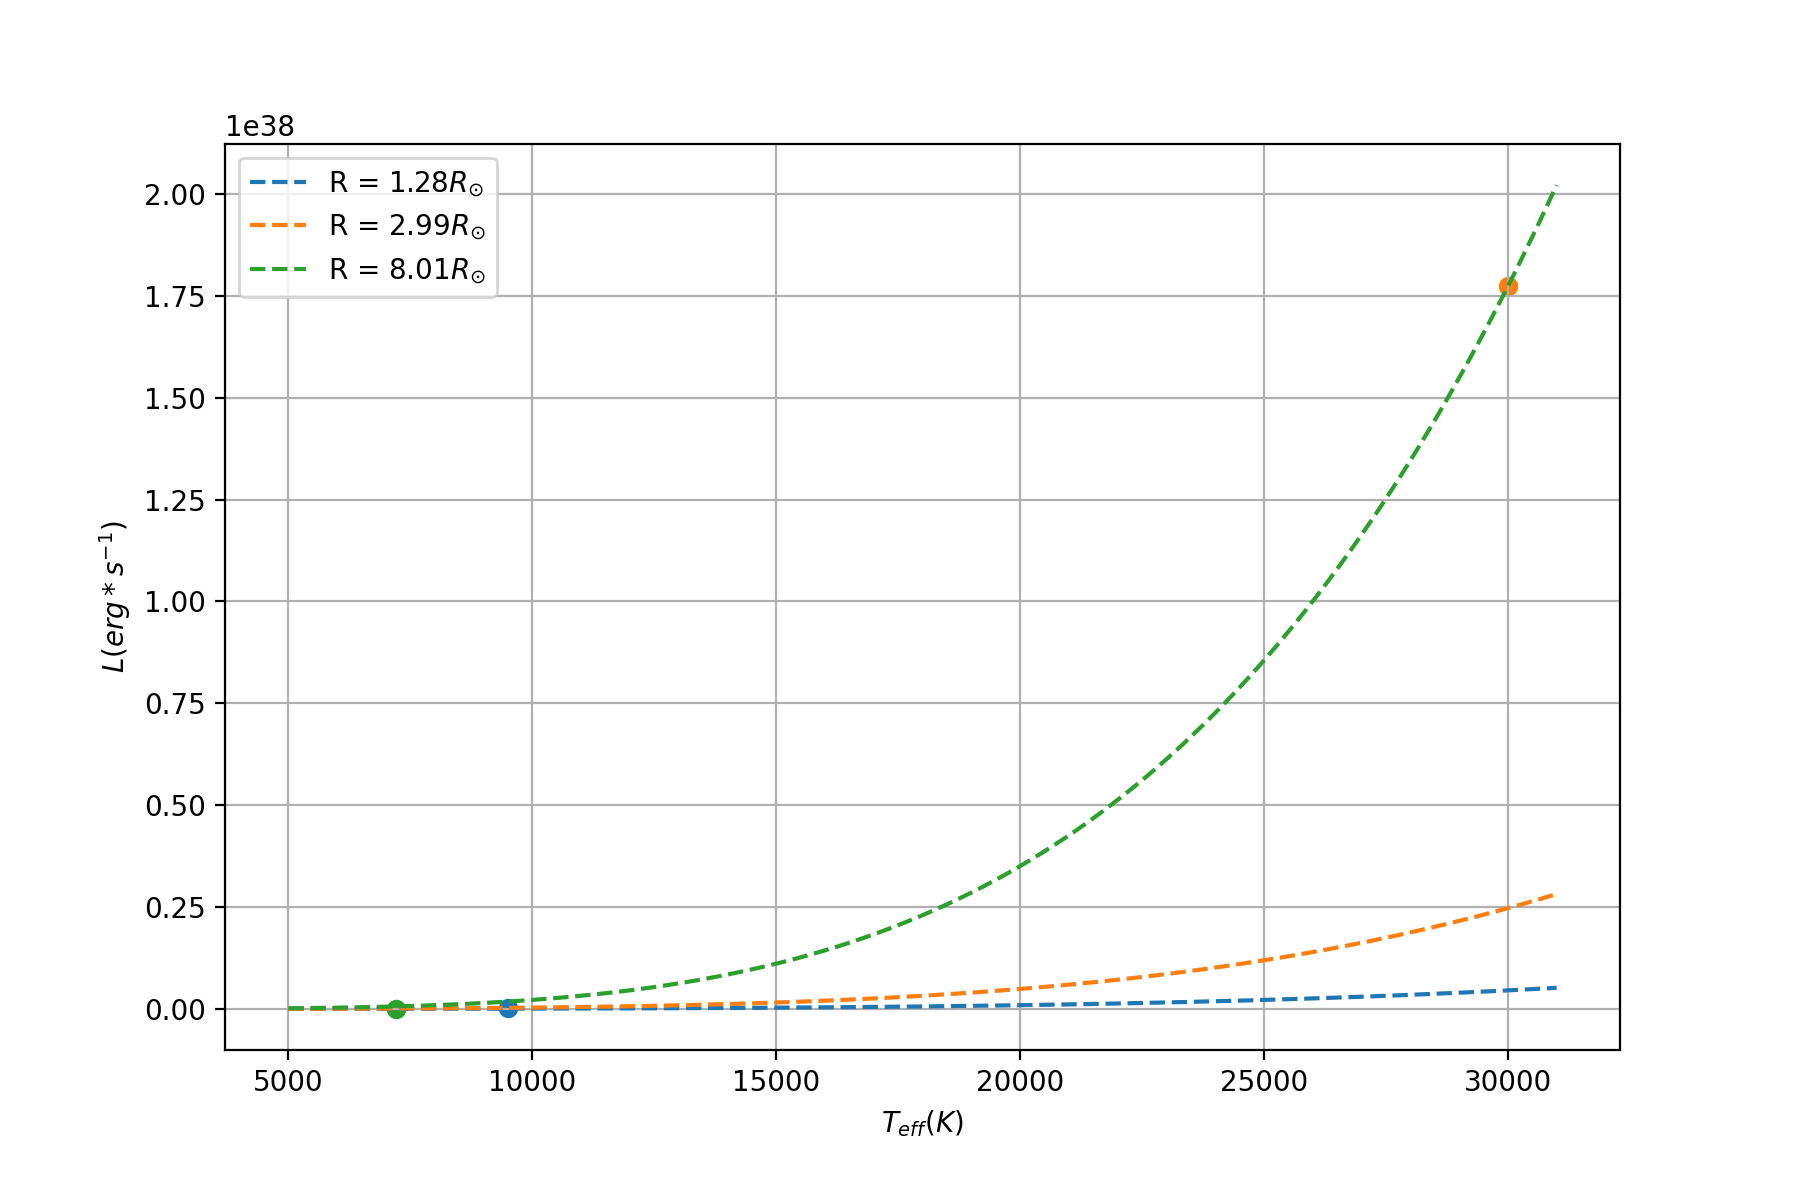
\includegraphics[scale=0.35]{TL.png}
\caption{Gráfica temperatura - luminosidad. Las curvas que aparecen son las curvas teóricas para la luminosidad en función de la temperatura que se esperarían para los radios de cada estrella en función de la ecuación \ref{eq:apuntes}}
\label{fig:TL}
\end{center}
\end{figure}

Se puede observar en esta gráfica como las tres estrellas se comportan de lo que se esperaría en función de la ecuación \ref{eq:apuntes}. Es una señal bastante fuerte de que los datos y la teoría están de acuerdo, aunque eso ya lo sabíamos gracias a la tabla \ref{table:spectral}.

A continuación, vamos a estudiar los espectros desenrojecidos de las dos estrellas problemas, estos son los que aparecen en la figura \ref{fig:desenrojecidos}. Lo que haremos será construir los espectros de emisión de un cuerpo negro ideal (figura \ref{fig:bbody}) en las temperaturas de las dos estrellas problema.

\begin{figure}[h!]
\begin{center}
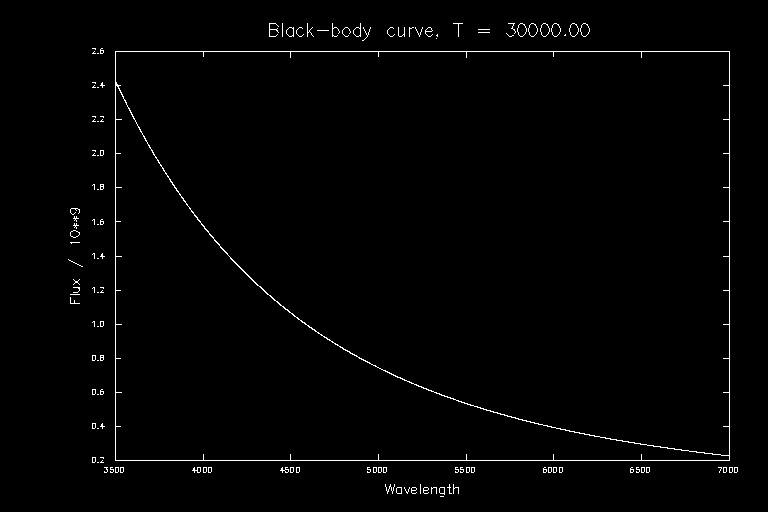
\includegraphics[scale=0.15]{bbody 30000.png}
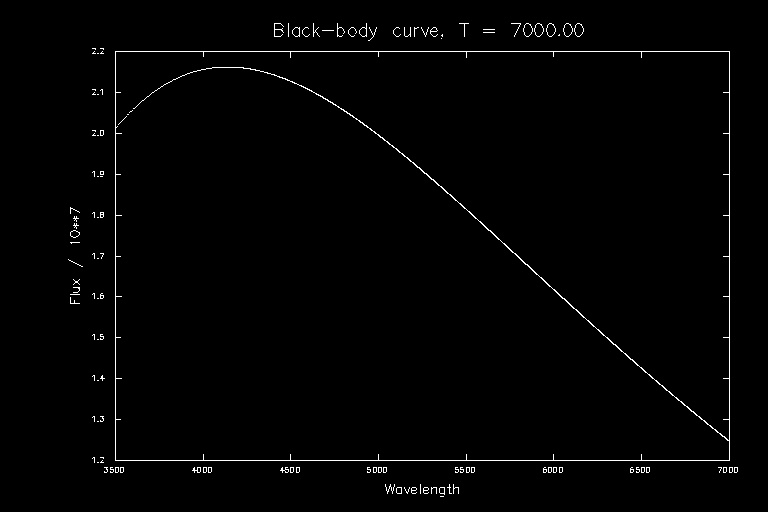
\includegraphics[scale=0.15]{bbody 7000.png}
\caption{Espectro de emisión de un cuerpo negro a 30000K y a 7000K.}
\label{fig:bbody}
\end{center}
\end{figure}

Vamos a comenzar comparando el espectro del cuerpo negro de 30000K con el espectro de la estrella 2, esto es lo que aparece en la figura \ref{fig:bbody2}.

\begin{figure}[h!]
\begin{center}
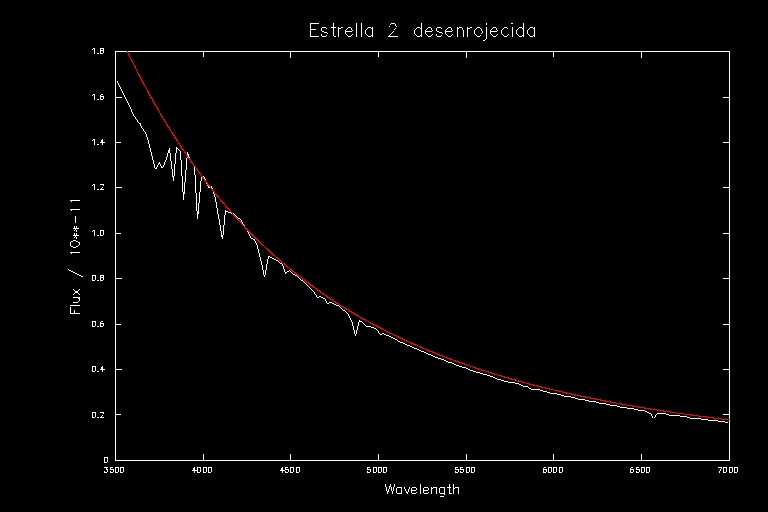
\includegraphics[scale=0.15]{2 bbody.png}
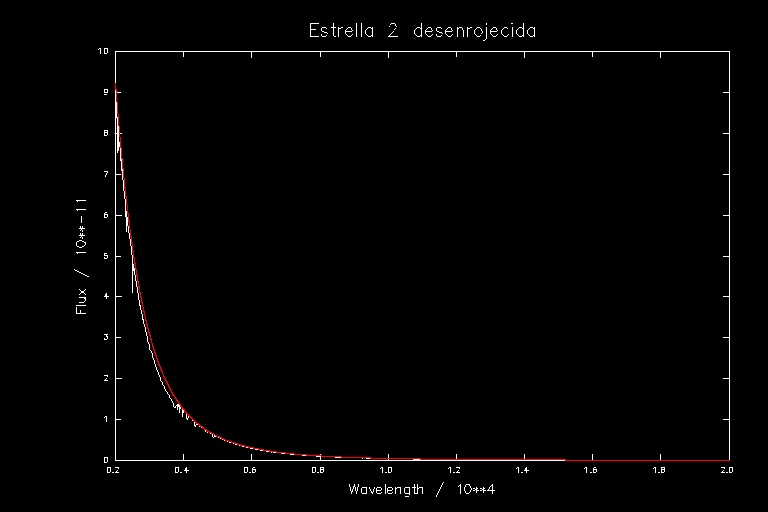
\includegraphics[scale=0.15]{2 bigger.png}
\caption{Comparación del espectro de emisión de la estrella 2 con el de un cuerpo negro de 30000K en dos rangos de longitudes de onda.}
\label{fig:bbody2}
\end{center}
\end{figure}

Para este caso podemos observar que la línea de emisión del cuerpo negro se pega muy bien a la de la estrella, incluso al aumentar el rango de longitudes de onda.

Cabe destacar esos picos hacia abajo que presenta la estrella respecto al cuerpo negro. Es evidente que una estrella no es un cuerpo negro ideal, por lo que no vamos a tener una línea perfecta. Estos picos que aparecen se deben a la composición química de la estrella. Distintos elementos presentan distintas líneas de absorción y por ello alguna luz de la estrella la observamos con menor intensidad.

Observemos ahora la comparación con la estrella 3 (figura \ref{fig:bbody3}).

\begin{figure}[h!]
\begin{center}
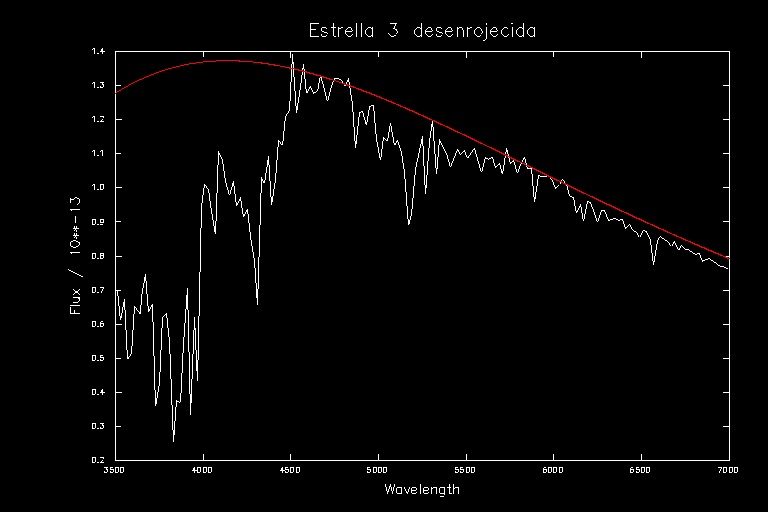
\includegraphics[scale=0.15]{3 bbody.png}
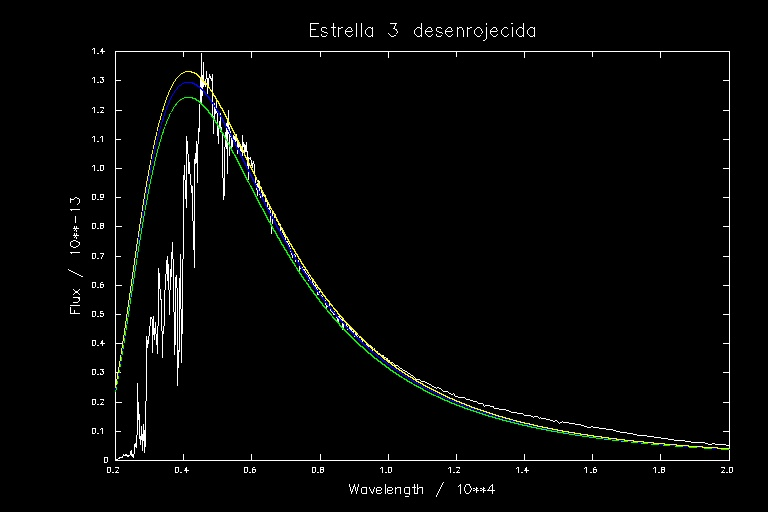
\includegraphics[scale=0.15]{3 bigger.png}
\caption{Comparación del espectro de emisión de la estrella 3 con el de un cuerpo negro de 7000K en dos rangos de longitudes de onda.}
\label{fig:bbody3}
\end{center}
\end{figure}

Observamos lo mismo que en el caso de la estrella dos, aunque en este caso el espectro de la estrella se parece mucho menos al cuerpo negro equivalente. Aun así, el modelo de cuerpo negro se aproxima bastante bien a la realidad de la estrella.

En la estrella problema 2 observamos lineas de absorción del helio y del hidrógeno que son las que veríamos en la estrella problema 2, mientras que en la estrella problema 3 podemos observar algunos metales en las líneas de absorción. (Estos elementos están tomados de la clasificación estelar de Harvard)

Aunque no podemos concluir que esta sea la composición química de la propia estrella en sí, pues el medio interestelar puede presentar nubes de gases o cualquier tipo de materia que puede generar absorción, así como la propia atmósfera del planeta Tierra. Como no sabemos el origen de nuestros datos no podemos descartar ningún efecto.

Finalmente, observemos la comparación del espectro de la estrella de ejemplo 1 con el de un cuerpo negro de la misma temperatura.

\begin{figure}[h!]
\begin{center}
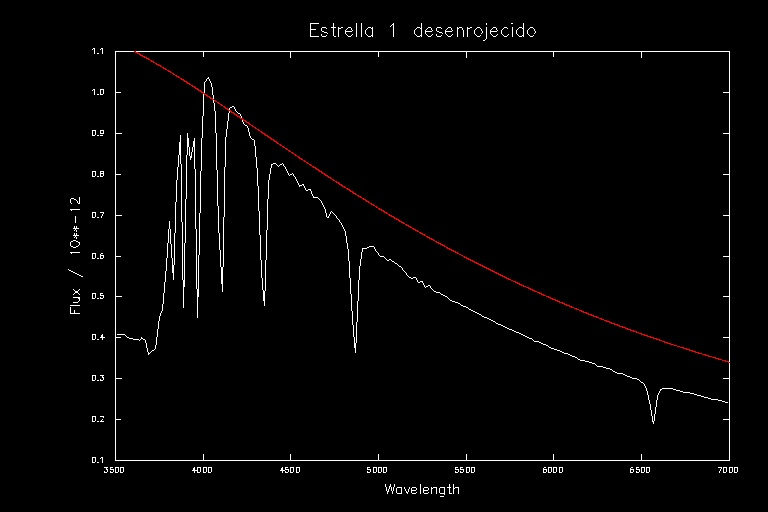
\includegraphics[scale=0.15]{1 bbody.png}
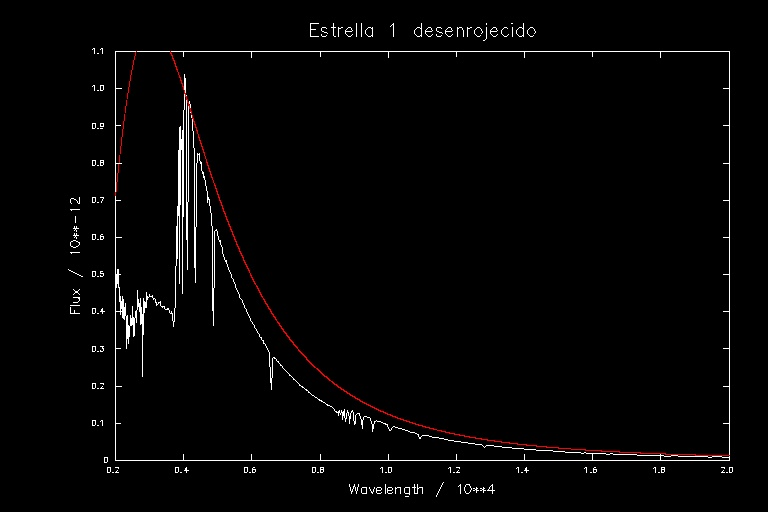
\includegraphics[scale=0.15]{1 bigger.png}
\caption{Espectro de la estrella de ejemplo 1 comparado con la de un cuerpo negro a la misma temperatura.}
\end{center}
\end{figure}

Donde en este caso la gráfica no se ajusta tan bien, al igual que sucedía en el problema 3.

\section{Conclusiones}

Con esta información podemos discernir lo correcto de nuestros datos, y es que, como hemos podido observar en la figura \ref{fig:TL} las tres estrellas se comportan como se esperaría de la teoría en la ecuación \ref{eq:apuntes}.

Queda entonces patente la utilidad de la espectroscopia para determinar propiedades de las estrellas. Ya sea su distancia o tamaño.

Vamos a intentar utilizar el catálogo de Simbad \cite{CiteDrive2022} para identificar las estrellas. En el caso de la estrella 3 encontramos varias estrellas que comparten tipo espectral y distancia con la estrella problema, aunque no tenemos ninguna medida del radio para cerrar más la búsqueda, ver la figura \ref{fig:simbad3}. Aunque ningún flujo coincide con el de nuestra estrella.

\begin{figure}[h!]
\begin{center}
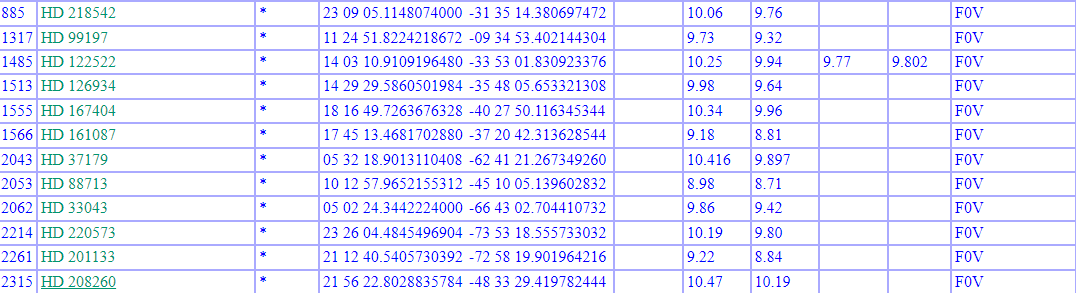
\includegraphics[scale=0.3]{simbad3.png}
\caption{Resultados de la busqueda en el catálogo Simbad para una distancia en los márgenes de nuestro error y que compartan tipo espectral con la estrella 3.}
\label{fig:simbad3}
\end{center}
\end{figure}

Para el caso de la estrella de ejemplo 1 la búsqueda en Simbad nos da 700 resultados que están en el rango de error de nuestra distancia y que comparten el tipo espectral por lo que no los puedo incluir en una imagen, pero \href{https://simbad.cds.unistra.fr/simbad/sim-sam?Criteria=Distance.distance+<%3D+720+%26+Distance.distance+>%3D+600+%26+sptype+%3D+%27A0V%27&submit=submit+query&OutputMode=LIST&maxObject=10000&CriteriaFile=}{dejo un enlace de la búsqueda.}

En el caso de la estrella 2 la búsqueda únicamente nos da tres resultados, con lo que podemos indagar un poco y ver si conseguimos identificar alguna de estas tres estrellas con la que tenemos problema.

\begin{figure}[h!]
\begin{center}
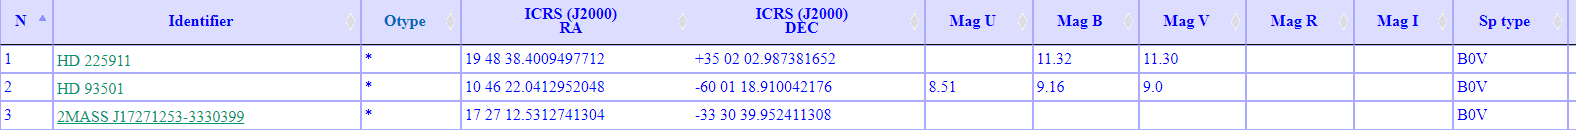
\includegraphics[scale=0.2]{simbad2.png}
\caption{Resultados de la búsqueda en el catálogo Simbad para la estrella 2.}
\end{center}
\end{figure}

Las estrellas candidatas que encuentra el catálogo son \href{https://simbad.cds.unistra.fr/simbad/sim-id?Ident=%402903109&Name=HD%20225911&submit=submit}{HD225911}, \href{https://simbad.cds.unistra.fr/simbad/sim-id?Ident=%403201202&Name=HD%20%2093501&submit=submit}{HD93501} y \href{https://simbad.cds.unistra.fr/simbad/sim-id?Ident=%408542189&Name=2MASS%20J17271253-3330399&submit=submit}{2MASS J17271253-3330399}.

En este caso la primera de estas estrellas la podemos descartar debido a que el flujo que marca \cite{CiteDrive2022} es mucho menor al que obtenemos nosotros, donde, $(B-V) = 0.97500 \pm 0.00001$ y la magnitud que observa en el catálogo es de $(B-V) = 0.02$ lo que es demasiado pequeña.

Haciendo una investigación sobre HD 93501 encontramos que esta estrella cumple muchos parámetros que cumple nuestra estrella problema. Observemos la referencia \cite{Richard_2018}, en ella se indica que esta estrella tiene los siguientes parámetros:

$$
\begin{array}{cc}
R = 7.96 \, R_{\odot} & L_{bol} = 44280
\end{array}
$$

Además el error que se da de estos parámetros en el artículo es lo suficientemente grande como para que entre en nuestros datos. La coincidencia de estos parámetros nos lleva a querer identificar la estrella problema 2 con esta estrella, sin embargo, vamos a investigar antes la tercera opción.

Sin embargo, al buscar referencias para esta estrella no logramos encontrar nada que nos permita identificarla con la estrella problema. Luego, finalmente concluimos que la estrella más similar en propiedades a la estrella problema es \textbf{HD 93501}.

Podremos finalmente cerrar el trabajo dejando como pincelada final que, por un lado, los datos son dentro de lo que cabe suficientemente correctos, sin embargo, se requiere más investigación para poder identificar cada estrella con una ya existente. No ayuda en esto que la estrella 1 tenga un margen de error tan alto.

Por otro lado, (exceptuando la estrella 1), los errores relativos son suficientemente pequeños como para ser aceptables.

Con este trabajo queda patente la utilidad de la espectrometría para la determinación de variables generales de algunas estrellas, llegando incluso a identificar la estrella 2 con una ya existente, gracias al catálogo de Simbad.

Como nota personal destacar que esta práctica es la que más me gustó de las de clase ya que tuvimos que usar varios conjuntos de habilidades obtenidos a lo largo de la carrera, por ejemplo, yo he usado Python para este trabajo y hojas de cálculo de Excel para ordenar los datos. Personalmente esta práctica me gustó y la volvería a hacer encantado.

\section{Anexo 1: fórmulas de errores}

Podemos dar una cota superior del error en el enrojecimiento utilizando la siguiente expresión:

$$
\Delta E(B-V) \leq 2.5 \left( \frac{\Delta f_V}{f_V} + \frac{\Delta f_B}{f_B} \right)
$$

Luego, el error en $A_V$ es directamente multiplicar el error en el enrojecimiento. Lo mismo con el error de $V_0$ que no es difícil de calcular.

Despejando la distancia tenemos que su error viene dado por la cota:

$$
\Delta d \leq \frac{ln(10)}{5} d \Delta V_0
$$

El error del radio a partir de la constante de normalización es directamente el error de la distancia en kiloparsecs, que es el del apartado anterior.

Para el error en la luminosidad obtenemos que:

$$
\Delta L(L_{\odot}) \leq 2R(R_{\odot}) \left( \frac{T_eff}{T_{\odot}} \right)^4 \Delta R (R_{\odot})
$$

\section{Anexo 2: el código}

En la entrega del informe debería de haber adjuntado un .zip en el que se incluyan los archivos para ejecutar el código Latex, así como el código de Python que he utilizado para generar la gráfica \ref{fig:TL} y las de comparación para el análisis del tipo espectral.

En todo caso, habré montado un repositorio en \href{https://github.com/luisgotsky}{mi perfil de GitHub} que se puede encontrar en el siguiente enlace y que contiene tanto el código Python como el código de Latex. 

\section{Anexo 3: tablas}

Adjunto todas las tablas de las fórmulas de Excel como capturas de pantalla aquí abajo.

\begin{figure}[h!]
\begin{center}
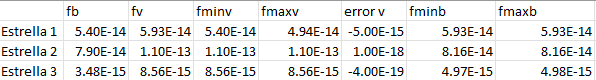
\includegraphics[scale=0.4]{tabla1.png}
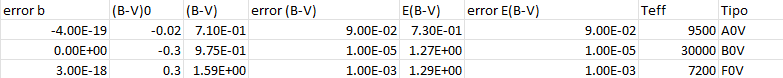
\includegraphics[scale=0.4]{tabla2.png}
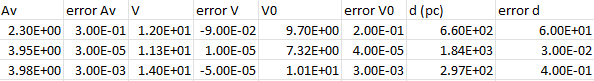
\includegraphics[scale=0.4]{tabla3.png}
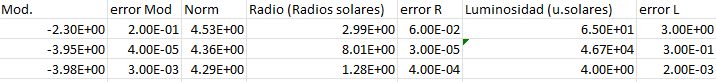
\includegraphics[scale=0.4]{tabla4.png}
\caption{Imágenes de las tablas de Excel para el informe.}
\end{center}
\end{figure}

Aun así, el Excel también se encuentra disponible para descargar en el repositorio de GitHub.

\bibliographystyle{aa} % style aa.bst
\bibliography{biblio.bib} % your referencesYourfile.bib
\end{document}